\documentclass[tikz,border=4pt]{standalone}
\usepackage{amsmath}
\begin{document}
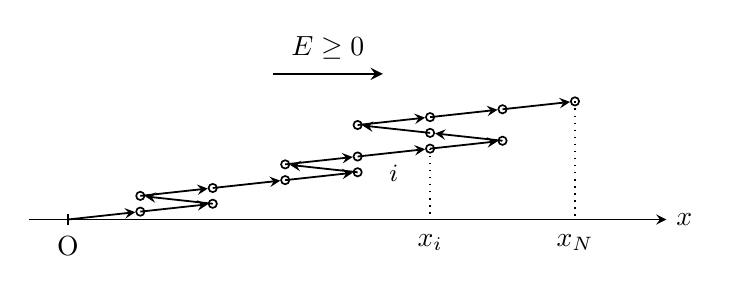
\begin{tikzpicture}[>=stealth, thick, scale=1.0]
  % x-axis
  \draw[->, line width=0.6pt] (-0.5, 0) -- (7.6, 0) node[right] {$x$};
  \draw[line width=0.6pt] (0, -0.07) -- (0, 0.07);
  \node[below] at (0, -0.08) {$\mathrm{O}$};

  % Electric field arrow above
  \draw[->, line width=0.95pt] (2.6, 1.85) -- (4.0, 1.85);
  \node[above] at (3.3, 1.90) {$E \ge 0$};

  % Zig-zag 1D polymer chain of equal horizontal step b = 0.9, slightly staggered in y for clarity
  % Steps (mu_i): +1, +1, -1, +1, +1, +1, -1, +1, +1, +1, -1, -1, +1, +1, +1
  \def\bstep{0.92}
  \def\dy{0.10}
  \coordinate (p0) at (0.0, 0.0);
  \coordinate (p1) at (1*\bstep, 1*\dy);
  \coordinate (p2) at (2*\bstep, 2*\dy);
  \coordinate (p3) at (1*\bstep, 3*\dy);
  \coordinate (p4) at (2*\bstep, 4*\dy);
  \coordinate (p5) at (3*\bstep, 5*\dy);
  \coordinate (p6) at (4*\bstep, 6*\dy);
  \coordinate (p7) at (3*\bstep, 7*\dy);
  \coordinate (p8) at (4*\bstep, 8*\dy);
  \coordinate (p9) at (5*\bstep, 9*\dy);
  \coordinate (p10) at (6*\bstep, 10*\dy);
  \coordinate (p11) at (5*\bstep, 11*\dy);
  \coordinate (p12) at (4*\bstep, 12*\dy);
  \coordinate (p13) at (5*\bstep, 13*\dy);
  \coordinate (p14) at (6*\bstep, 14*\dy);
  \coordinate (p15) at (7*\bstep, 15*\dy);

  % Draw arrows for each segment and small open circles for charges Q at tips
  \foreach \a/\b in {p0/p1, p1/p2, p2/p3, p3/p4, p4/p5, p5/p6, p6/p7, p7/p8, p8/p9, p9/p10, p10/p11, p11/p12, p12/p13, p13/p14, p14/p15} {
    \draw[->, line width=0.65pt, shorten >=1.8pt] (\a) -- (\b);
    \draw[line width=0.6pt] (\b) circle (1.5pt);
  }

  % Label i-th segment (p8 -> p9) and its tip coordinate x_i, plus endpoint x_N
  \node[below, font=\small] at (4.5*\bstep, 8.2*\dy) {$i$};
  \draw[dotted, line width=0.55pt] (p9) -- (5*\bstep, 0);
  \node[below] at (5*\bstep, -0.06) {$x_i$};

  \draw[dotted, line width=0.55pt] (p15) -- (7*\bstep, 0);
  \node[below] at (7*\bstep, -0.06) {$x_N$};
\end{tikzpicture}
\end{document}
